\section{Benchmarking the~AWBS nonlocal transport model}
\label{sec:BenchmarkingAWBS}
After having shown several encouraging properties of the~AWBS transport 
equation defined by \eqref{eq:AWBS_model} under local diffusive conditions
in \secref{sec:DiffusiveKinetics}, this section provides a~broader analysis
of the~electron transport and focuses on analysis its behavior under variety of
conditions in plasmas. In principle, this is characterized by allowing that
electron mean free path can be arbitrarily long, which leads to so-called 
nonlocal electron transport extensively investigated in numerous publications 
\cite{Malone_1975_15, Colombant_PoP2005, Bell_1981_83, LMV_1983_7, Brantov_Nonlocal_electron_transport_1998, schurtz2000, Sorbo_2015}, where the~Fokker-Planck
modeling of electrons in plasma represents the~essential tool. Being so, 
we introduce our implementation of the~AWBS transport equation called AP1,
where its results are further benchmarked against simulation results
provided by Aladin, Impact VFP codes, and Calder a~collisional Particle-In-Cell
code. Their description follows in the~next section.

\subsection{Implementation of the~model}
\label{sec:C7code}

Here, we use the~collision operator \eqref{eq:AWBS_model} with 
\eqref{eq:qAWBS_approximation} and the~P1 angular discretization 
referred to as AP1. It adopts the~so-called angular 
moments method with the~electron distribution function having the~form
\begin{equation}
  \tilde{\ft} = \frac{\fzero}{4\pi} + \frac{3}{4\pi}\vn\cdot\fone , 
  \label{eq:P1approximation}
\end{equation}
which consists of the~isotropic part represented by the zeroth angular moment 
$\fzero = \int_{4\pi} \tilde{\ft} \dI\vn$ 
and the~directional part represented by the~first angular moment 
$\fone = \int_{4\pi} \vn
\tilde{\ft} \dI\vn$, where $\vn$ is the~transport direction (the~solid angle).
It should noticed, that \eqref{eq:P1approximation} represents 
a~multi-dimensional equivalent to \eqref{eq:f_approximation}, where 
the~following relations between the~spherical harmonics method
and the~moments method hold $\ft^0 = \frac{\fzero}{4\pi}$ and 
$\ft^1 = \frac{3}{4\pi}|\fone|$.

The~first two angular moments applied to the~steady form of 
\eqref{eq:kinetic_equation} with collision operator \eqref{eq:AWBS_model} 
using \eqref{eq:qAWBS_approximation} lead to the~AP1 model equations
\begin{eqnarray}
  \vmag\frac{\nue}{2}\pdv{}{\vmag}\left(\fzero - 4\pi\fM \right) &=&
  \vmag\nabla\cdot\fone + \frac{\qe}{\me}\E\cdot\left(
  \pdv{\fone}{\vmag} + \frac{2}{\vmag}\fone\right) , 
  \nonumber \\
  \label{eq:AP1f0}\\
  \vmag\frac{\nue}{2}\pdv{\fone}{\vmag}
  - \nuscat\fone &=& 
  \frac{\vmag}{3}\nabla\fzero + 
  \frac{\qe}{\me}\frac{\E}{3}\pdv{\fzero}{\vmag} ,
  \label{eq:AP1f1}
\end{eqnarray}
where $\nuscat = \nuei + \frac{\nue}{2}$. The~strategy of solving 
\eqref{eq:AP1f0} and \eqref{eq:AP1f1} resides in integrating 
$\pdv{\fzero}{\vmag}$
and $\pdv{\fone}{\vmag}$ along the~velocity magnitude. 
This is done by starting the~integration
from infinite velocity ($\vmag = 7 \vth^{max}$) to zero velocity. The~value
$\vth^{max}$ equals the~electron thermal velocity corresponding to the~maximum 
electron temperature in the~current profile of plasma.
It should be noted, that the~backward integration concept is crucial for 
the~model, since it corresponds to the~deceleration of electrons due to 
collisions \cite{Touati_2014}. 

\begin{figure}[tbh]
  \begin{center}
    \begin{tabular}{c}
      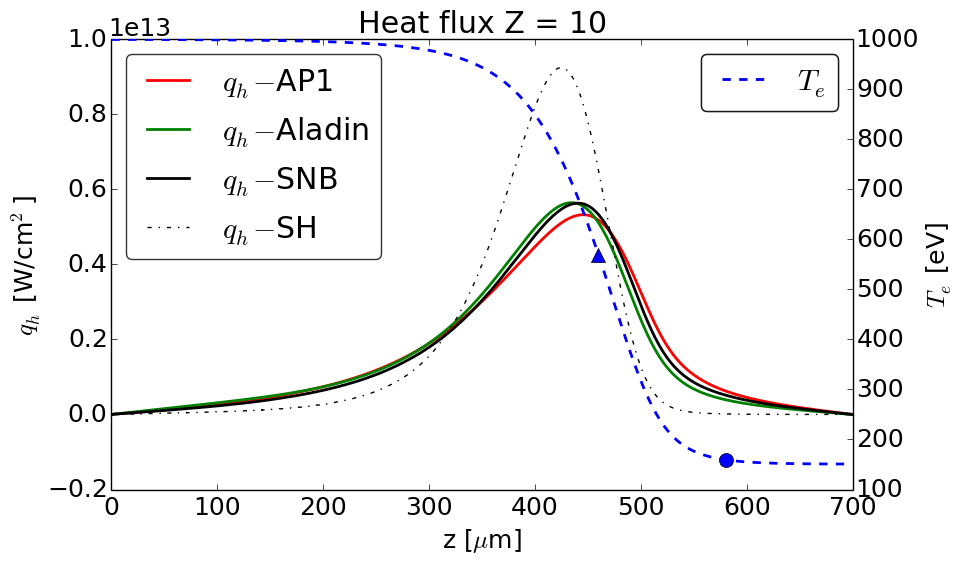
\includegraphics[width=\figscale\textwidth]{../VFPdata/C7_Aladin_case3_heatflux.png} \\
      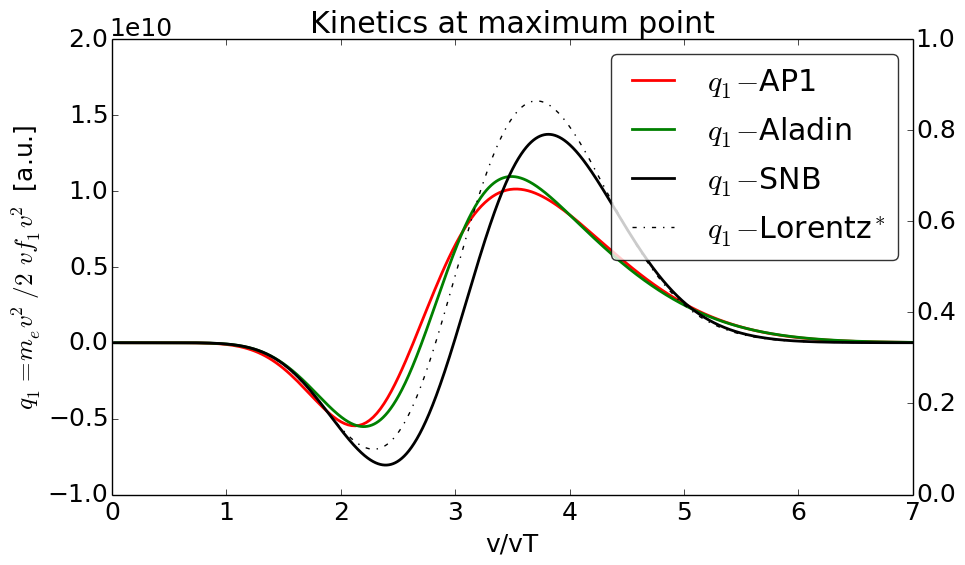
\includegraphics[width=\figscale\textwidth]{../VFPdata/C7_Aladin_case3_kinetics.png}
    \end{tabular}
  \caption{  
  Snapshot 12 ps. Left: correct steady solution of heat flux. 
  Right: correct comparison to kinetic profiles at point 442 $\mu$m by Aladin. 
  Velocity limit 3.4 $\vth$.
  }
  \label{fig:C7_Aladin_case3}
  \end{center} 
\end{figure}


\subsubsection{Nonlocal electric field treatment}
\label{sec:Efield}

%\begin{multline}
%  %\frac{\vect{j}}{\qe} = 
%  \vect{q}_c \equiv
%  \qe \intv \Bigg[\frac{\frac{\nue}{2}\vmag^2}{\nuei + \frac{\nue}{2}}
%  \pdv{\fone}{\vmag} 
%  - \frac{\vmag^2}{3\left(\nuei + \frac{\nue}{2}\right)}
%  \nabla\fzero \\
%  - \frac{\vmag}{3\left(\nuei + \frac{\nue}{2}\right)}\pdv{\fzero}{\vmag}\tE
%  \Bigg] \vmag^2\, \dI\vmag = 0
%  , \nonumber
%\end{multline}
Similarly to the~quasi-neutrality condition \eqref{app_eq:BGK_Efield}, 
one can obtain the~model equation of the~electric field $\E$ by evaluating 
the~zero current condition (a~first moment velocity integration of 
\eqref{eq:AP1f1})
\begin{equation}
  \intv \left(\frac{\frac{\nue}{2}\vmag^2}{\nuscat}
  \pdv{\fone}{\vmag} 
  - \frac{\vmag^2}{3\nuscat}
  \nabla\fzero 
  - \frac{\vmag}{3\nuscat}\pdv{\fzero}{\vmag}\frac{\qe}{\me}\E
  \right) \vmag^2\, \dI\vmag = 0 ,
  \label{eq:AP1_Efield}
\end{equation}
from which it is easy to express $\E$ once $\fzero$ and $\fone$ are known.

In other words, the~integral-differential model equations 
\eqref{eq:AP1f0}, \eqref{eq:AP1f1}, and \eqref{eq:AP1_Efield}
need to be solved simultaneously. This is achieved by $k$-iteration of 
$\fzero^k(\E^k), \fone^k(\E^k)$, i.e. \eqref{eq:AP1f0}, \eqref{eq:AP1f1}, and 
$\E^{k+1}(\fzero^k, \fone^k)$, i.e.  \eqref{eq:AP1_Efield}, until 
the~current evaluation \eqref{eq:AP1_Efield} converges to zero. In principle,
our concept of $k$-iteration resembles to the~embedded nonlinear iteration
of the~implicit E field introduced in \cite{Kingham_JCP2004}.
The~first iteration starts with $\E=\vect{0}$ in \eqref{eq:AP1f0} and 
\eqref{eq:AP1f1} and usually less than 10 iterations is sufficient to obey
the~quasi-neutrality constraint.
%\begin{eqnarray}
%  \pdv{\fzero}{\vmag} &=&
%  \frac{2}{\nue}\pdv{\fonez}{z} + \frac{2\Ez}{\vmag\nue} \pdv{\fonez}{\vmag} 
%  + \frac{4}{\vmag^2\nue}\Ez\fonez 
%  + 4\pi\pdv{\fM}{\vmag}
%  , \nonumber\\
%  \vmag\frac{\nue}{2}\pdv{\fonez}{\vmag} 
%  &=&  
%  \frac{\Ez}{3}\pdv{\fzero}{\vmag} + \frac{\vmag}{3}\pdv{\fzero}{z} 
%  + \left(\nuei + \frac{\nue}{2}\right)\fonez
%  , \nonumber \label{eq:OOE_P1f1}
%\end{eqnarray}

Interestingly, we have encountered a~very specific property of the~AP1 model
with respect to the~electric field magnitude. The~easiest way how to 
demonstrate this is to write the~model equations \eqref{eq:AP1f0} and 
\eqref{eq:AP1f1} in 1D (z-axis). Then, due to its linear nature, it is easy 
to eliminate one of the~partial derivatives with respect to $\vmag$, i.e. 
$\pdv{\fzero}{\vmag}$ or $\pdv{\fonez}{\vmag}$. 
In the~case of elimination of $\pdv{\fzero}{\vmag}$ 
one obtains the~following equation
\begin{multline}
  %\frac{2}{3\vmag\nue} 
  %\left(\left(\sqrt{3}\vmag\frac{\nue}{2}\right)^2 - \Ez^2\right)  
  \left(\vmag\frac{\nue}{2} - \frac{2\qe^2\Ez^2}{3\me^2\vmag\nue}\right) 
  \pdv{\fonez}{\vmag} 
  =
  \frac{2\qe\Ez}{3\me\nue}\pdv{\fonez}{z}  
  + \frac{4\pi\qe\Ez}{3\me}\pdv{\fM}{\vmag} \\
  + \frac{\vmag}{3}\pdv{\fzero}{z} 
  + \left(\frac{4\qe^2\Ez^2}{3\me^2\vmag^2\nue}
  + \left(\nuei + \frac{\nue}{2}\right) \right)\fonez .
  \label{eq:AP1_model_1D}
\end{multline}
It is convenient to write the~bracket on the~left hand side of 
\eqref{eq:AP1_model_1D} as
$\frac{2}{3\vmag\nue} 
\left(\left(\sqrt{3}\vmag\frac{\nue}{2}\right)^2 
- \frac{\qe^2}{\me^2}\Ez^2\right)$
from where it is clear that the~bracket is negative if 
$\sqrt{3}\vmag\frac{\nue}{2} < \frac{\qe}{\me}|\E|$, 
i.e. there is a~velocity limit for a~given magnitude $|\E|$, 
when the~collisions are no more fully dominant and the~electric field 
introduces a~comparable effect to the~collision friction in 
the~electron transport.

It can be shown, that the~last term on the~right hand side of 
\eqref{eq:AP1_model_1D} is dominant and the~solution behaves as 
\begin{equation}
  \Delta \fone \sim \exp\left(\frac{\frac{4\qe^2\Ez^2}{3\me^2\vmag^2\nue}
  + \left(\nuei + \frac{\nue}{2}\right)}
  {\vmag\frac{\nue}{2} - \frac{2\qe^2\Ez^2}{3\me^2\vmag\nue}}\, 
  \Delta\vmag\right) ,
  \label{eq:f1z_behavior}
\end{equation}
where $\Delta \vmag < 0$ represents a~velocity step of the~implicit Euler
numerical integration of decelerating electrons.
However, \eqref{eq:f1z_behavior} exhibits an~exponential growth 
for velocities above the~friction limit (bracket on the~left hand side of 
\eqref{eq:AP1_model_1D})
\begin{equation}
  \vmag_{lim}  = \sqrt{\frac{\sqrt{3}\Gamma\me}{2\qe}\frac{n_e}{|\E|}} ,
  \label{eq:v_limit}
\end{equation}
which makes the~problem to be ill-posed.

%\begin{table}
%\begin{center}
%  \begin{tabular}{c|ccccc}
%    \hline\hline\\
%    Kn$^e$ & $\,\,10^{-3}\,\,$ & $\,\,5\times10^{-3}\,\,$ & $\,\,10^{-2}\,\,$ & $\,\,5\times10^{-2}\,\,$ & $\,\,10^{-1}\,\,$ \\\\
%    \hline\\
%    $\vmag_{lim}^{Z=1} / \vth$ & 21.6 & 9.8 & 7.0 & 3.8 & 3.1 \\\\
%    \hline\\
%    $\vmag_{lim}^{Z=2} / \vth$ & 14.8 & 6.8 & 5.0 & 3.1 & 2.6 \\\\
%    \hline\\
%    $\vmag_{lim}^{Z=10} / \vth$ & 6.7 & 3.4 & 2.6 & 1.6 & 1.3 \\\\
%    \hline\hline
%  \end{tabular}
%  \caption{
%  $\sqrt{3}\vmag\frac{\nue}{2} > |\tE|$.
%  }
%\end{center}
%\label{tab:vlim}
%\end{table}

\begin{table}
\begin{center}
  \begin{tabular}{c|ccccc}
    \hline\hline\\
    %Kn$^e$ & $10^{-4}$ & $10^{-3}$ & $10^{-2}$ & $10^{-1}$ & $1$ \\\\
    Kn$^e$ & $\,\,10^{-4}\,\,$ & $\,\,10^{-3}\,\,$ & $\,\,10^{-2}\,\,$ & $\,\,10^{-1}\,\,$ & $\,\,1\,\,$ \\\\
    \hline\\
    $\vmag_{lim} / \vth$ & 70.8 & 22.4 & 7.3 & 3.1 & 1.8\\\\
    \hline\hline
  \end{tabular}
  \caption{
  $\sqrt{3}\vmag\frac{\me}{2\qe}\nue > |\E|$.
  }
\label{tab:vlim}
\end{center}
\end{table}

In order to provide a~stable model, we introduce a~reduced electric field
to be acting as the~accelerating force of electrons
\begin{equation}
  |\E_{red}| = \sqrt{3} \vmag\frac{\me}{2\qe}\nue ,
  \label{eq:Elimit}
\end{equation}
ensuring that the~bracket on the~left hand side of \eqref{eq:AP1_model_1D}
remains positive. Further more we define two quantities
\begin{equation}
  \omega_{red} = \frac{|\E_{red}|}{|\E|} ,\quad 
  \nuscat^E = \frac{\qe}{\me\vmag} \left(|\E| - |\E_{red}|\right),
  \nonumber
\end{equation}
introducing the~reduction factor of the~electric field
$\omega_{red}$ and the~compensation of the~electric field effect in terms of
scattering $\nuscat^E$. Consequently, the~AP1 model \eqref{eq:AP1f0}, 
\eqref{eq:AP1f1}, and \eqref{eq:AP1_Efield} can be formulated as well posed 
with the~help of $\omega_{red}$ and $\nuscat^E$. Nevertheless, before doing so,
we introduce a~slightly different approximation to the~electron distribution 
function as
\begin{equation}
  \tilde{f} = \frac{4\pi \fM + \dafzero}{4\pi} + \frac{3}{4\pi}\vn\cdot\fone .
  \label{eq:P1_OOE}
\end{equation}
where $\dafzero$ represents the~departure of isotropic part from 
the~Maxwell-Boltzmann equilibrium distribution $\fM$. 
%which we keep 
%intentionally in the~distribution function approximation.
Then, the~stable AP1 model reads
\begin{eqnarray}
  \vmag \frac{\nue}{2}\pdv{\dafzero}{\vmag} &=&
  \vmag\nabla\cdot\fone 
  + \frac{\qe}{\me}\E\cdot\left(\omega_{red} \pdv{\fone}{\vmag} 
  + \frac{2}{\vmag}\fone\right) , 
  \label{eq:AP1f0_stable}\\
  \vmag\frac{\nue}{2}\pdv{\fone}{\vmag} 
  &=& \tnuscat\fone 
  + \frac{\vmag}{3}\nabla\left(4\pi\fM + \dafzero\right)
  \nonumber \\
  && 
  + \frac{\qe\E}{3\me}\left(4\pi \pdv{\fM}{\vmag} 
  + \omega_{red} \pdv{\dafzero}{\vmag} 
  \right) ,
  \label{eq:AP1f1_stable}
\end{eqnarray}
where $\tnuscat = \nuei + \nuscat^E + \frac{\nue}{2}$.

The~reason for keeping $\fM$ in the~distribution function approximation
\eqref{eq:P1_OOE} can be seen in the~last term on the~right hand side of 
\eqref{eq:AP1f1_stable}, which provides the~effect of electric field on
directional quantities as current or heat flux. In principle, the~explicit use
of $\fM$ ensures the~proper effect of $\E$ if $\dafzero \ll \fM$, i.e.
no matter what the~reduction $\omega_{red}$ is. Apart from its stability,
it also exhibits much better convergence of the~electric field, which is now
given by the~zero current condition of \eqref{eq:AP1f1_stable} as
\begin{equation}
  \E =
  \frac{\intv \left(\frac{\nue}{2\tnuscat}\vmag^2\pdv{\fone}{\vmag}
  - \frac{\vmag^2}{3\tnuscat}
  \nabla\left(4\pi\fM + \dafzero\right)\right) \vmag^2\, \dI\vmag}
  {\frac{\qe}{\me}\intv \frac{\vmag}
  {3\tnuscat}
  \left(4\pi\pdv{\fM}{\vmag} + \omega_{red} \pdv{\dafzero}{\vmag}\right)
  \vmag^2\, \dI\vmag} .
  \label{eq:AP1_Efield_stable}
\end{equation}

For practical reasons we present in \tabref{tab:vlim} 
some explicit values of velocity limit corresponding to varying transport 
conditions expressed in terms of "$\Zbar$" Knudsen number 
$\text{Kn}^e = \frac{\mfpe}{\sqrt{\Zbar + 1}L_{T_e}}$, 
where $\sqrt{\Zbar + 1}$ provides a~proper scaling of nonlocality with respect
to ionization, i.e. the~effect of scattering of electrons on ions 
\cite{LMV_1983_7}.

\begin{figure}[tbh]
  \begin{center}
    \begin{tabular}{c}
      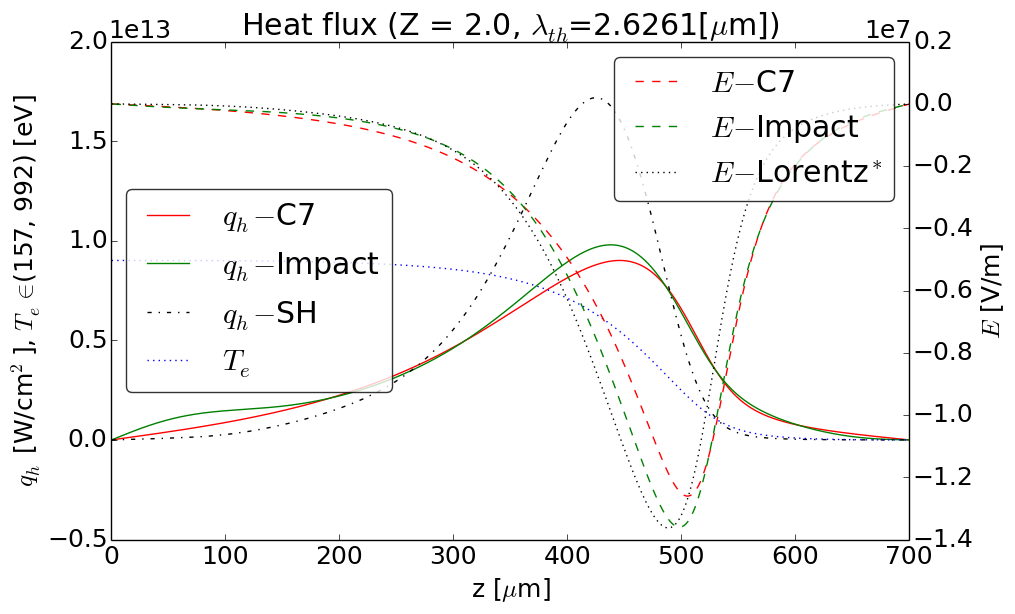
\includegraphics[width=\figscale\textwidth]{../VFPdata/C7_Impact_case3_heatflux.png} \\
      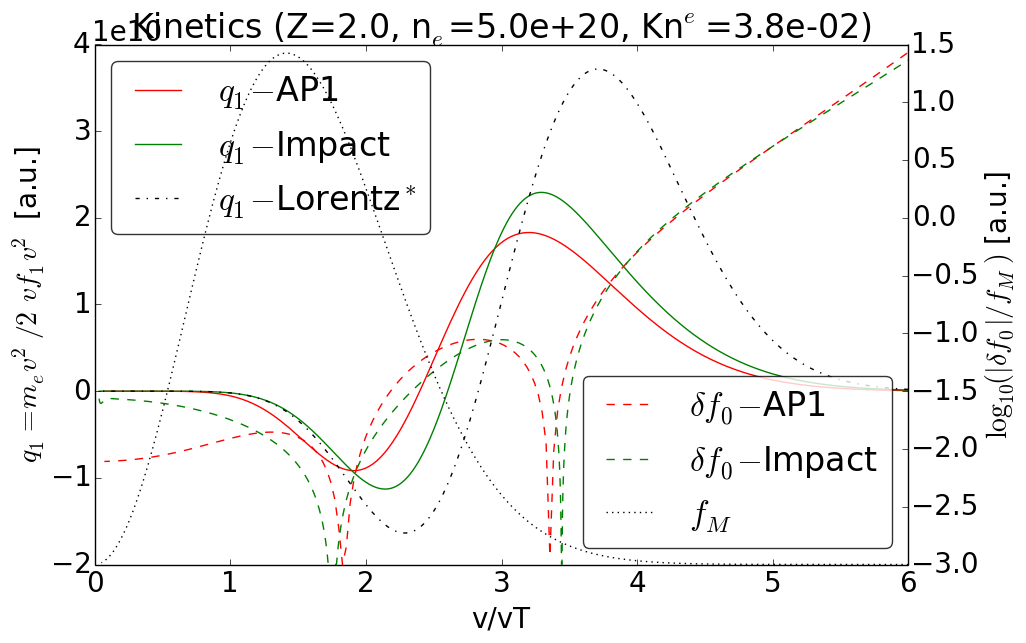
\includegraphics[width=\figscale\textwidth]{../VFPdata/C7_Impact_case3_kinetics.png}
    \end{tabular}
  \caption{  
  Snapshot 12 ps. Left: correct steady solution of heat flux. 
  Right: correct comparison to kinetic profiles at point 437 $\mu$m by Impact.
  Velocity limit 4.0 $\vth$.
  }
  \label{fig:C7_Impact_case3}
  \end{center} 
\end{figure}

\subsection{Aladin, Impact, and Calder kinetic codes}
\label{sec:AladinImpactCaldercodes}

\begin{itemize}
  \item Brief description of the Aladin code \figref{fig:C7_Aladin_case5}, \figref{fig:C7_Aladin_case3}. %\figref{fig:C7_Aladin_case6}
\end{itemize}

\begin{itemize}
  \item Brief description of the Impact code \figref{fig:C7_Impact_case3}.
\end{itemize}

\begin{figure}[tbh]
  \begin{center}
    \begin{tabular}{c}
      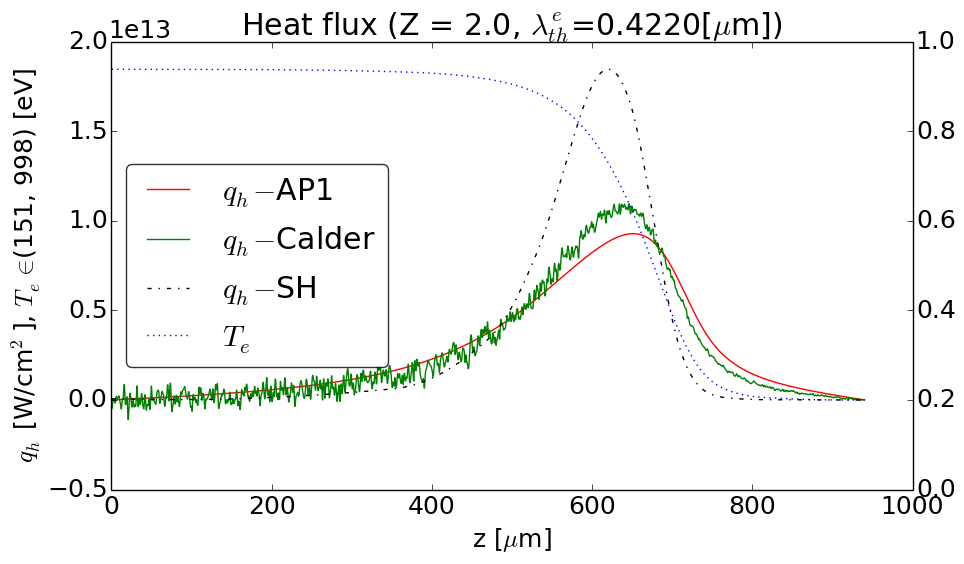
\includegraphics[width=\figscale\textwidth]{../VFPdata/C7_Calder_case1_heatflux.png} 
	  %\\ 
	  %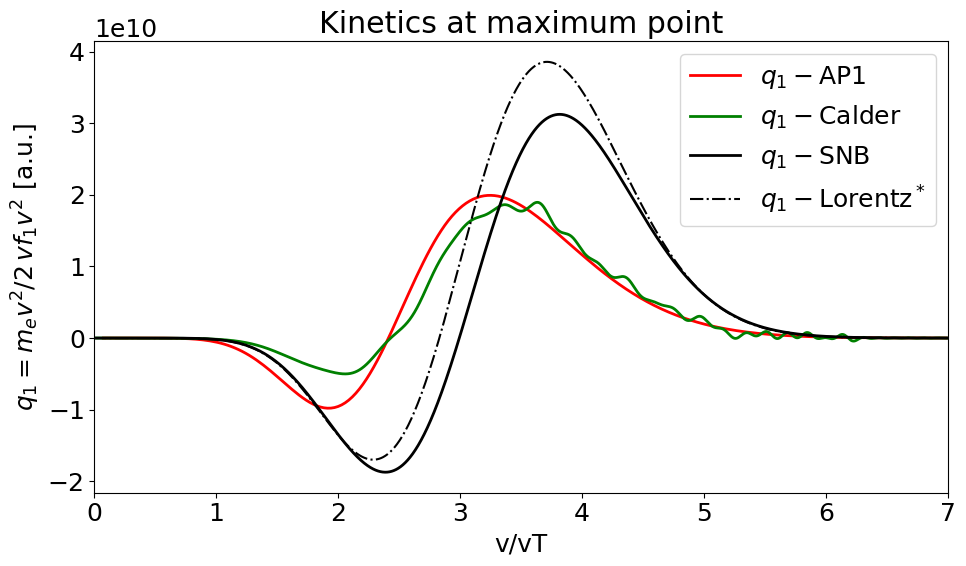
\includegraphics[width=\figscale\textwidth]{../VFPdata/C7_Calder_case1_kinetics.png}
    \end{tabular}
  \caption{  
  Snapshot 11 ps. Left: correct steady solution of heat flux. 
  %Right: AP1 kinetic profiles at point 750~$\mu$m corresponding to 
  %a~highly nonlocal nature of the~heat flux and is in a~good agreement with
  %\cite{Sherlock_PoP2017}. Velocity $max(q_1)$ = 5.8 $\vth$. 
  Velocity limit 6.4 $\vth$.
  }
  \label{fig:C7_Calder_case1}
  \end{center} 
\end{figure}

\begin{itemize}
  \item Brief description of the Calder code \figref{fig:C7_Calder_case1}.
\end{itemize}

\subsection{Tests relevant to laser-heated plasmas}
\label{sec:SimulationResults}

Among a~variety of test suitable for benchmarking the~nonlocal electron 
transport models published 
\cite{Epperlein_PoFB1991, marocchino2013, Sorbo_2015, 
Sorbo_2016, Sherlock_PoP2017, Brodrick_PoP2017}, we decided to focus on 
conditions relevant to inertial confinement fusion plasmas generated by lasers.

%\subsubsection{Heat-bath problem}  
%\label{sec:heatbath_test}
%\begin{figure}[tbh]
%  \begin{center}
%    \begin{tabular}{c}
%      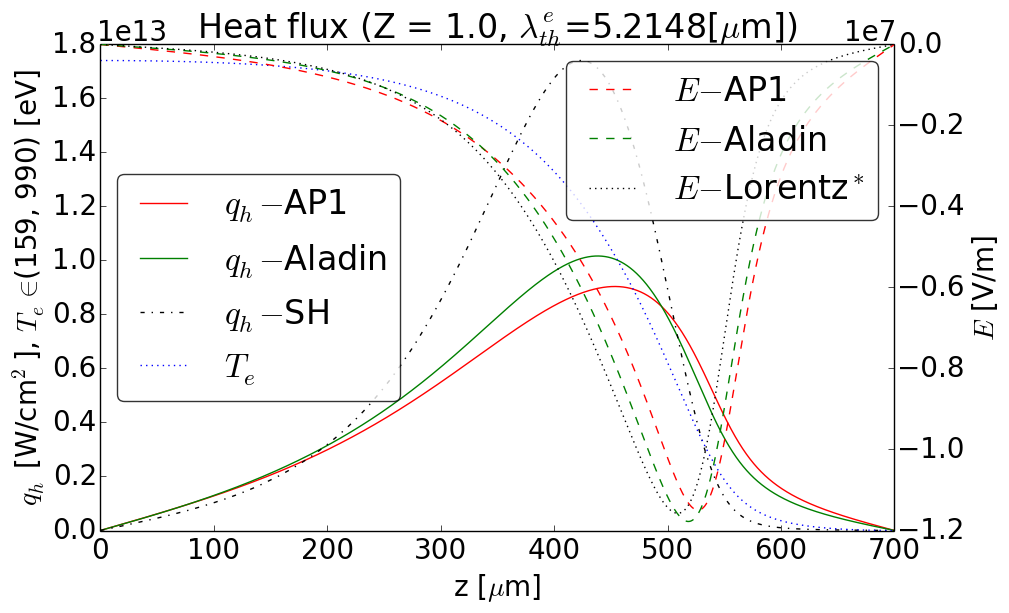
\includegraphics[width=\figscale\textwidth]{../VFPdata/C7_Aladin_case5_heatflux.png} \\
%      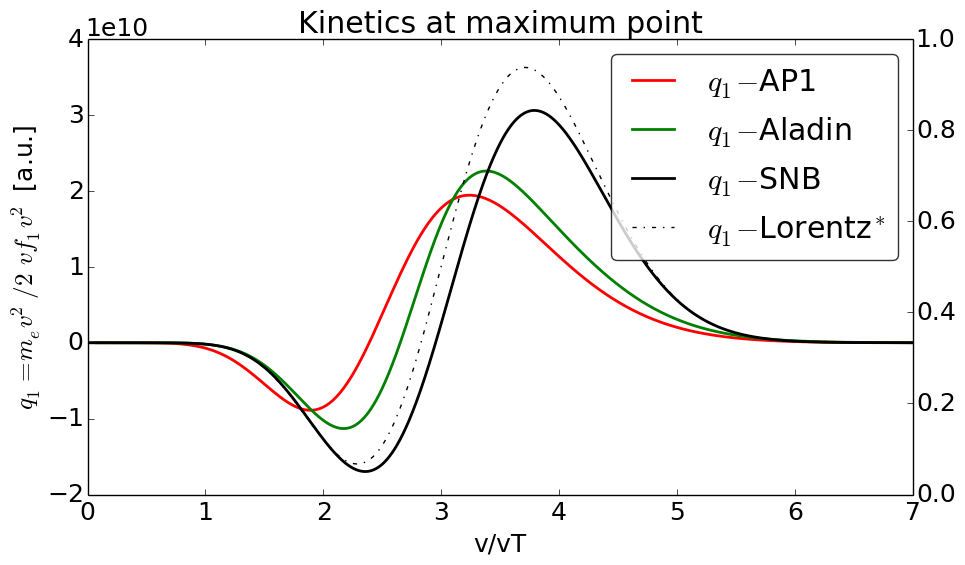
\includegraphics[width=\figscale\textwidth]{../VFPdata/C7_Aladin_case5_kinetics.png}
%    \end{tabular}
%  \caption{  
%  Snapshot 20 ps. Left: correct steady solution of heat flux. 
%  Right: Aladins results are correct. Velocity limit 4.4 $\vth$..
%  }
%  \label{fig:C7_Aladin_case5}
%  \end{center} 
%\end{figure}
\begin{figure}[tbh]
  \begin{center}
    \begin{tabular}{c}
      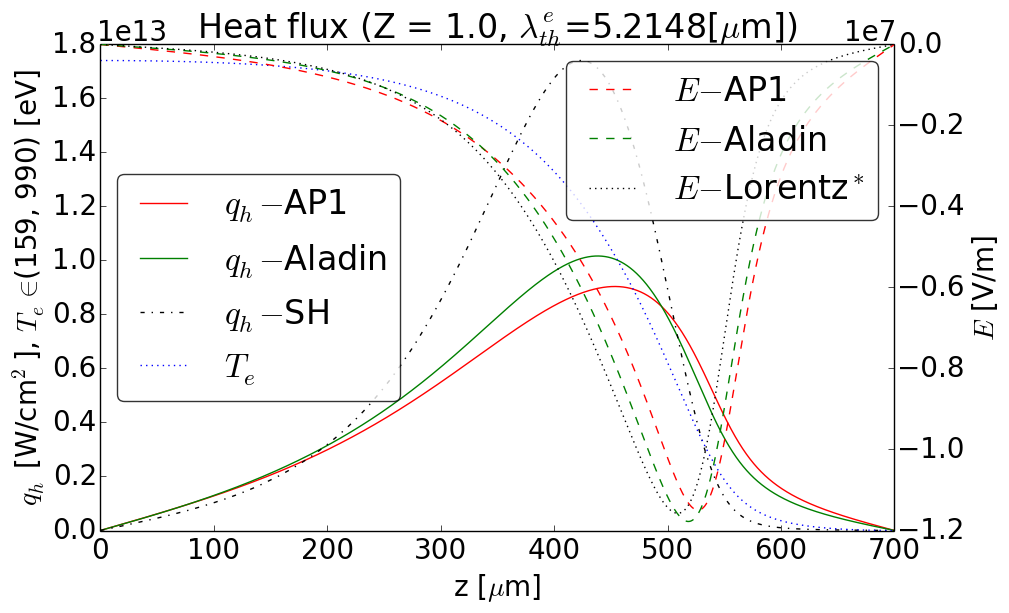
\includegraphics[width=\figscale\textwidth]{../VFPdata/C7_Aladin_case5_heatflux.png} \\
      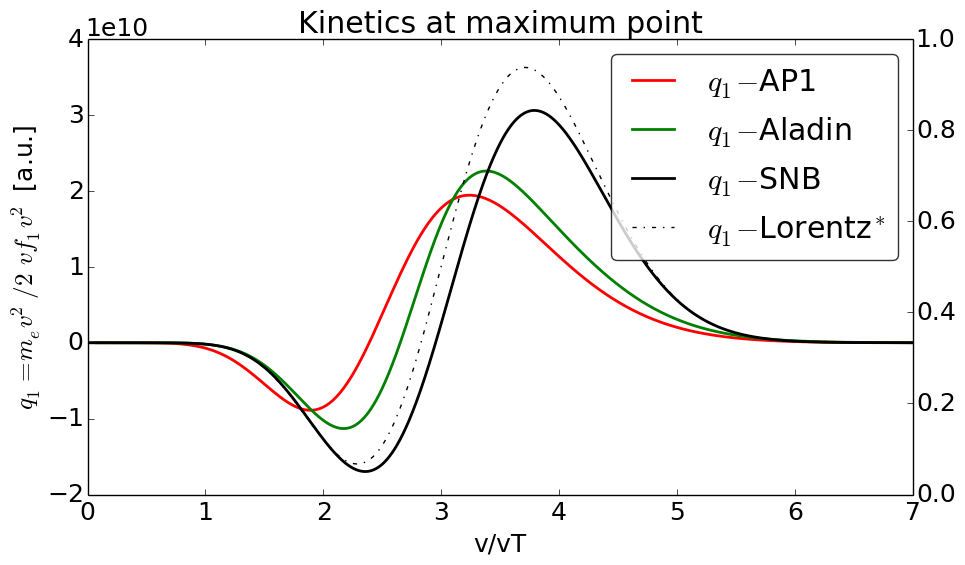
\includegraphics[width=\figscale\textwidth]{../VFPdata/C7_Aladin_case5_kinetics.png} \\
	  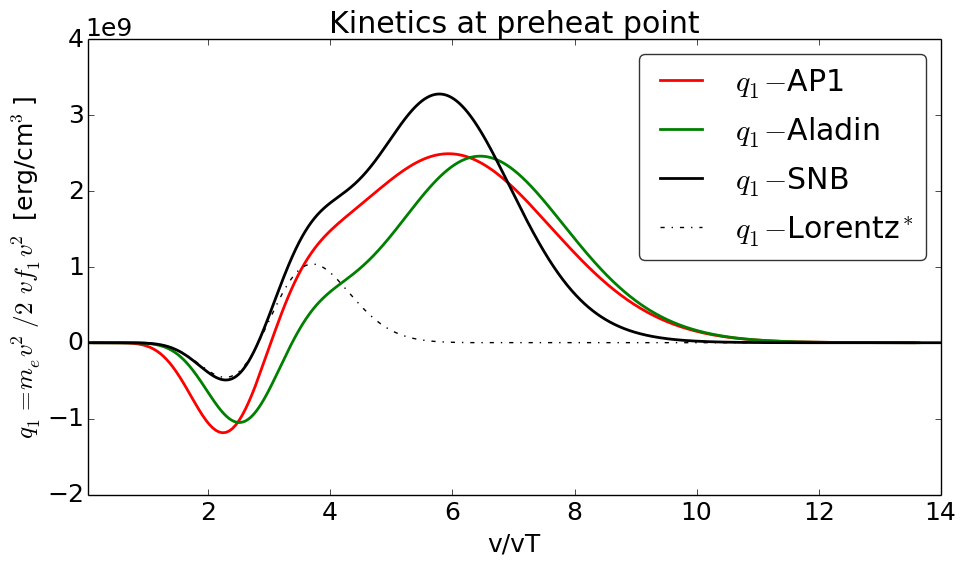
\includegraphics[width=\figscale\textwidth]{../VFPdata/C7_Aladin_case5_nonlocal_kinetics.png}
    \end{tabular}
  \caption{  
  Snapshot 20 ps. Left: correct steady solution of heat flux. 
  Right: Aladins results are correct. Velocity limit 4.4 $\vth$.
  Snapshot 20 ps. AP1 kinetic profiles at point 580~$\mu$m corresponding to 
  a~highly nonlocal nature of the~heat flux %\figref{fig:C7_Aladin_case5} 
  and is in a~good agreement with
  \cite{Sherlock_PoP2017}. Velocity $max(q_1)$ = 6.0 $\vth$. 
  Velocity limit 9.0 $\vth$.
  }
  \label{fig:C7_Aladin_case5}
  %\label{fig:C7_Aladin_case5_nonlocal}
  \end{center} 
\end{figure}

The accuracy of the AP1 implementation is compared to Aladin, Impact and Calder
codes by calculating the heat flow in the case
where a~large relative temperature variation
\begin{equation}
  T_e(z) = 0.575 - 0.425 \tanh\left((z-450) s\right) ,
  \label{eq:T_init}
\end{equation}
which exhibits a~smooth steep gradient at point 450~$\mu$m 
connecting a~hot bath ($T_e = 1$~keV) 
and cold bath ($T_e = 0.17$~keV) and $s$ is the~parameter of steepness. 
This test is referred to as a~simple non-linear heat-bath problem and
originally was introduced in \cite{marocchino2013} and further investigated
in  \cite{Sorbo_2015, Sorbo_2016, Sherlock_PoP2017, Brodrick_PoP2017}.

%Aladin and Impact simulations showed an evolution of the heat flow
%from the local (due to initialising as a Maxwellian) to the
%nonlocal, with a reduced peak, over an initial transient
%phase (over which the temperature ramp flattened somewhat). 
%The transient phase was considered over when the
%ratio of the VFP heat flow to the expected local heat
%flow stopped decreasing. After the transient phase this
%ratio begins to slowly increase as the thermal conduction flattens 
%the temperature ramp and the ratio of the scalelength to mfp increases 
%(i.e. the thermal transport slowly becomes more local). 

The~total computational box size is 700 $\mu$m in the~case
of Aladin and Impact and 1000 $\mu$m in the~case of Calder.
We performed Aladin, Impact, and Calder simulations showing an~evolution of
temperature starting from the~initial profile \eqref{eq:T_init}. 
Due to an~inexact initial distribution function (approximated by Maxwellian),
the~first phase of the~simulation exhibits a~transient behavior of the~heat
flux. After several ps the~distribution adjusts properly to its nonlocal nature
and the~actual heat flux profile can be compared. 
We then take the temperature profile from Aladin/Impact/Calder and used 
our AP1 implementation to calculate the heat flow
it would predict given this profile. In~particular, the~AP1 results 
corresponding to the~evolved temperature profile by Aladin can be found
in \figref{fig:C7_Aladin_case5} and \figref{fig:C7_Aladin_case3} for 
$\Zbar = 1$ and $\Zbar = 10$ respectively. The~AP1 results computed on
the~evolved temperature profile for $\Zbar = 2$ by Impact are shown in 
\figref{fig:C7_Impact_case3} and by Calder can be found in 
\figref{fig:C7_Calder_case1}.

For all heat-bath simulations the electron density, Coulomb logarithm and 
ionisation were kept constant and uniform.
The~coulomb logarithm was held fixed throughout, 
$\lnc = 7.09$.
Nevertheless, the~Knudsen number Kn$^e$ has been varied among the~simulation 
runs in order to address a~broad range of nonlocality of 
the~electron transport corresponding 
to the~laser-heated plasma conditions, i.e. Kn$^e \in (0.0001, 1)$. 
The~variation of Kn$^e$ arises from the~variation
of the~uniform electron density $n_e \in (10^{19}, 10^{23})$ cm$^{-3}$ or 
the~length scale given by the~slope of the~temperature profile 
$s \in (1/2500, 1/25) \mu$m. Results of an~extensive set of simulations of
varying Kn$^e$ is shown in \figref{fig:Kn_results}.
 
\begin{figure}[tbh]
  \begin{center}
    \begin{tabular}{c}
      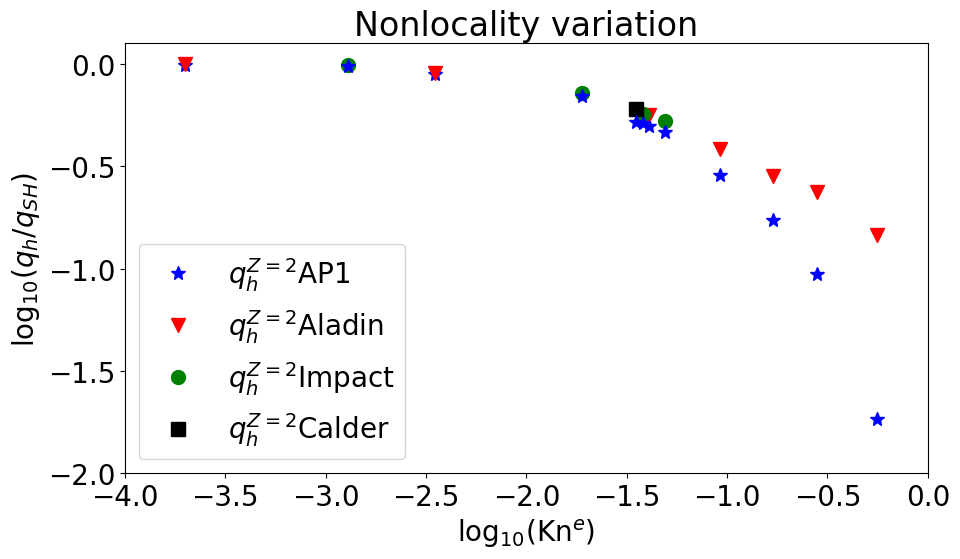
\includegraphics[width=\figscale\textwidth]{Kn_results.png}
    \end{tabular}
  \caption{  
  Simulation results for the case $Z=2$ computed by AP1/Aladin/Impact/Calder.
  Every point corresponds to the maximum heat flux in a "tanh" temperature 
  simulation, which can be characterized by Kn. The range of 
  $\log_{10}(\text{Kn})\in (0, -4)$ can be expressed as equivalent 
  to the~electron density approximate range n$_e \in (1e19, 3.5e22)$ of 
  the~50 $\mu$m slope tanh case. In the case of Kn = 0.56, 
  $q_{Aladin} / q_{AP1}\approx 7.9$.}
  \label{fig:Kn_results}
  \end{center} 
\end{figure}

Apart from the~distribution function details related to the~point of 
the~heat flux maximum, in \figref{fig:C7_Aladin_case5}
we also present the~detail of the~kinetic profile at point 580~$\mu$m 
corresponding to a~highly nonlocal nature of the~heat flux profile. 
Here a~good agreement with \cite{Sherlock_PoP2017} can be found.

In every simulation run of AP1 we used 250~velocity groups in order to avoid
numerical errors in modeling of the~electron kinetics. However, a~smaller 
number of groups, e.g. 50, provides a~very similar results 
(an~error around 10$\%$ in the~heat flux).

\subsubsection{Hohlraum problem}
%While comparisons between the AP1 model and VFP
%codes have previously been performed 8,45 , none have included 
%spatially-inhomogeneous ionisation. 
Additionally to the~steep temperature gradients, the~laser-heated plasma 
experiments also involve steep density gradients and variation in ionization,
which is even more dominant in multi-material targets as in inertial
fusion experiments, e.g. at the interface between the helium gas-fill and 
the ablated high $\Zbar$ plasma.
%, it is critical that the AP1 model be tested 
%in such an environment.

In~\cite{Brodrick_PoP2017}, a~kinetic simulation of such a~test was introduced.
Plasma profiles provided by a~HYDRA simulation in 1D spherical
geometry of a~laser-heated gadolinium hohlraum containing a~typical helium 
gas-fill were used as input for the~IMPACT \cite{Kingham_JCP2004} VFP code. 
Electron temperature $T_e$, electron density $n_e$ and ionisation $\Zbar$ 
profiles shown in \figref{fig:Gd_VFP_10ps_heatflux} at 20 nanoseconds of 
the~HYDRA simulation were used (after spline smoothing) as 
the~initial conditions for the~IMPACT run (in planar geometry). 
For simplicity, the Coulomb logarithm was treated as a
constant $\lnc_{ei}$ = $\lnc_{ee}$ = 2.1484. In reality, in the~low-density 
corona $\lnc$ reaches 8, which, however, does not affect the~heat flux profile 
significantly. 
%Note that in reality
%5the plasma is only strongly coupled in the colder region of
%the gadolinium bubble beyond $\sim$1.7 mm and $\lnc_{ei}\approx$ 8
%up to $\sim$1.6 mm in the hotter corona.

It is worth mentioning that in the~surroundings of the~heat flux maximum 
($\sim 1662 \mu$m) the~profiles of all plasma variables exhibit steep gradients 
with a change from $T_e$ = 2.5 keV, $n_e$ = 5$\times$10$^{20}$ cm$^{−3}$, 
$\Zbar$ = 2 to $T_e$ = 0.3 keV, $n_e$ = 6$\times$10$^{21}$ cm$^{−3}$ , 
$\Zbar$ = 44 across approximately 100 $\mu$m 
(between 1600~$\mu$m and 1700~$\mu$m), starting at the~helium-gadolinium 
interface.  

%Reflective boundary
%conditions were used here as in the previous section and
%IMPACT used a timestep of 1.334 fs. The $n_e$ and $\Zbar$ profiles did not 
%evolve in the IMPACT simulation due to the treatment of the electric field 
%discussed in section II that ensures quasineutrality and the neglection of 
%ion motion and ionisation models.

%As with the VFP simulations in the previous section,
%there is an initial transient phase where the IMPACT
%heat flux gradually reduces from the Braginskii prediction
%as the distribution function rapidly moves away from
%Maxwellian. Once again this transient phase is considered
%to be over when the ratio of the peak heat flow to the
%Braginskii prediction stops reducing. This ratio is not
%observed to change by more than 5\% after the first 5 ps
%of our 15.7 ps simulation. Therefore, we conclude that
%it safe to assume the transient phase is over after 5 ps,
%at which point the temperature front has advanced by
%approximately 8 $\mu$m leading to a maximum temperature
%change of 41\% as shown in \figref{fig:Gd_VFP_10ps_heatflux}.

%In comparing the IMPACT, AP1, and SNB heat flow profiles
%we encountered an important subtlety concerning the implementation of 
%the model. A~recent SNB model with separate electron
%ion and electron-electron collision frequencies provides a
%very good prediction of the preheat into the hohlraum, the
%peak heat flow to within 16\% and an improved estimate
%of the thermal conduction in the gas-fill region, the latter
%is still too large by a factor of $\sim$2. This discrepancy could
%potentially lead to an overestimate of hohlraum temperatures and thus cause 
%issues similar to those arising with
%using an overly restrictive flux limiter.

\begin{figure}[tbh]
  \begin{center}
    \begin{tabular}{c}
      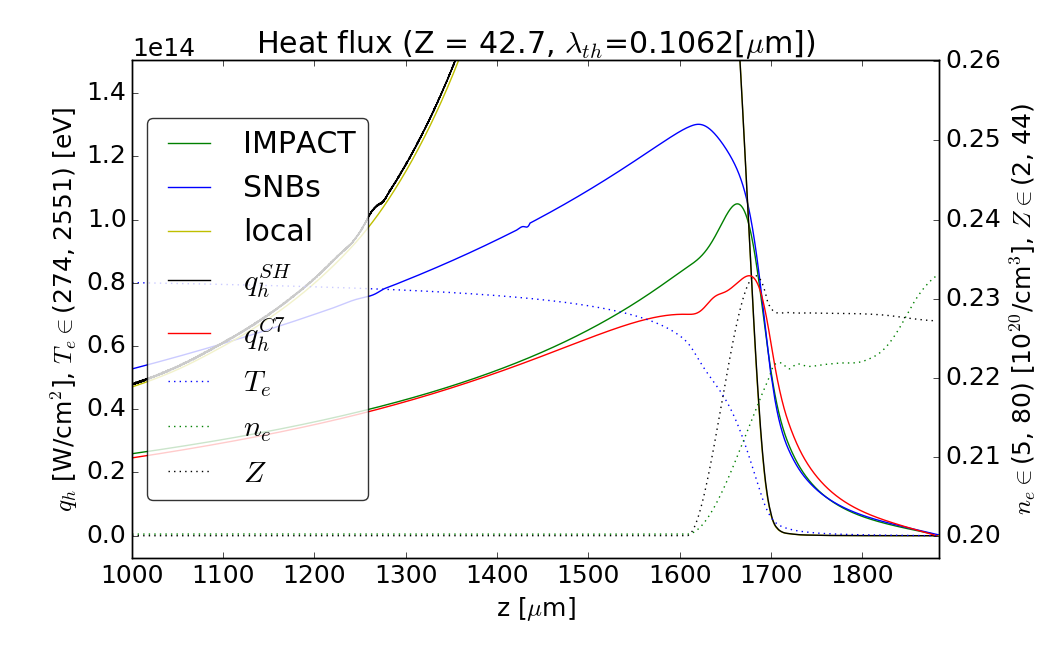
\includegraphics[width=\figscale\textwidth]{../VFPdata/GD_Hohlraum/fluxes_10ps.png} 
    \end{tabular}
  \caption{
  }
  \label{fig:Gd_VFP_10ps_heatflux}
  \end{center} 
\end{figure}

%\begin{itemize}
%  \item Multiple runs analyzing the~performance of AP1 with respect to 
%    Aladin/Impact/Calder along wide range of Kn$^e$ shown in 
%    \figref{fig:Kn_results}.
%  \item Realistic hydro simulation setting provided by HYDRA, a~comparison
%    between AP1, Impact, and SNB shown in \figref{fig:Gd_VFP_10ps_heatflux}.
%  \item Comment on and summarize the~velocity limits for all figs.
%\end{itemize}

%
